\documentclass[newpage,hints,handout]{ximera}

%\usepackage{microtype}
%\usepackage{tikz}
\usepackage{tkz-euclide}
%\usetkzobj{all}
\tikzstyle geometryDiagrams=[rounded corners=.5pt,ultra thick,color=blue!50!black]

\usepackage{tikz-cd}

\colorlet{penColor}{blue!50!black} % Color of a curve in a plot

%% \hypersetup{
%%     colorlinks = false,
%%     }


\tikzset{%% partial ellipse
    partial ellipse/.style args={#1:#2:#3}{
        insert path={+ (#1:#3) arc (#1:#2:#3)}
    }
}

\graphicspath{
{./}
{sphericalLunesAndTriangles/}
{hyperbolicLunesAndTriangles/}
{centralProjection/}
{stereographicProjection/}
{linesAnglesAndAreasInCentralProjection/}
{linesAnglesAndAreasInStereographicProjection/}
{stereographicProjection/}
{centralProjectionInHG/}
{stereographicProjectionInHG/}
{linesInSphericalGeometry/}
{linesInHyperbolicGeometry/}
{theArtOfEscher/}
}


\newcommand{\transpose}{\intercal}
\newcommand{\eval}[1]{\bigg[ #1 \bigg]}

\renewcommand{\epsilon}{\varepsilon}
\renewcommand{\l}{\ell}
\renewcommand{\d}{\,d}

\DeclareMathOperator{\arccosh}{arccosh}
\DeclareMathOperator{\arctanh}{arctanh}
\renewcommand{\tilde}{\widetilde}
\newcommand{\R}{\mathbb R}
\newcommand{\dd}[2][]{\frac{d #1}{d #2}}
\newcommand{\pp}[2][]{\frac{\partial #1}{\partial #2}}
\newcommand{\dfn}{\textbf}

\renewcommand{\bar}{\overline}
\renewcommand{\hat}{\widehat}


\ifxake
\NewEnviron{freeResponse}{}
\fi


\title{The upper half plane and hyperbolic triangles}

\begin{document}
\begin{abstract}
In this activity, we explore rigid motions of the upper half plane model, revisit the axioms of neutral geometry, and find the areas of polygons in hyperbolic geometry.
\end{abstract}
\maketitle


\section{Upper half plane model}

To work with hyperbolic space, we want a model that we can draw and look at. We cannot create a model that preserves lengths of geodesics and angles between curves. This is similar to how we cannot draw spherical geometry on a flat plane without distorting lengths or angles, but spherical geometry has the nice feature of working on spheres.

There are several models for hyperbolic geometry, but one of the most common is \emph{the upper half plane $\mathbb{H}=\{x+iy|y>0\}$}

You can get a sense of the upper half plane model of hyperbolic space by drawing in the GeoGebra applet \url{https://www.geogebra.org/m/dqc3uKhY#material/DBXvbruR}

\begin{problem}
 Using the GeoGebra applet, describe what the following look like in hyperbolic geometry:
 
\begin{itemize}
 \item Lines between two points
 \item Circle centered at some point
 \item Triangles
\end{itemize}
\end{problem}

\begin{definition}
  A \emph{geodesic} is in $\mathbb{H}$ is either a semicircle meeting the real axis
at right angles (ie, a circle centered on the x-axis), or a vertical ray emanating from a point on the real axis. 
\end{definition}

\begin{definition}
 The \emph{angle} between two geodesics is defined to be the angle between
the tangents to the geodesics at their intersection point. 
\end{definition}

\begin{definition}
 Let $p$ and $q$ be two points in $\mathbb{H}$. Let $o$ and $r$ denote the points
where the geodesic meets the real axis, as in Figure .
We define
\[distance(p, q) =\left|\ln\frac{|o-p||p-r|}{|o-q||q-r|}\right|\]
Here $|o - p|$ computes the Euclidean distance from $o$ to $p$. Likewise for the
other terms.
When $p$ and $q$ lie on the same vertical segment, we interpret $r = \infty$. In
this case, the second two factors cancel out, and the distance is:
\[distance(p, q) =\left|\ln\frac{|o-p|}{|o-q|}\right|.\]  To save space, we will write this function as $d_{hyp}$.
\end{definition}

\begin{definition} 
Let $f:\mathbb{H}\to\mathbb{H}$. Such a mapping is called a \emph{rigid motion of hyperbolic space} if the distance between any two points in hyperbolic space is left unchanged by the mapping, that is, for any two points $X_1$ and $X_2$ in hyperbolic space, \[d_{hyp}(X_1,X_2)=d_{hyp}(f(X_1),f(X_2)).\]
\end{definition}

\begin{problem}
 Let $z=x+iy, y>0$. Show that the following maps are rigid motions of hyperbolic space:
 
\begin{itemize}
\item Let $t$ be any real number and $f(z) = z +t$.
\item Let $t$ be a positive real number and $f(z) = tz$.
\item $f(x+iy)=-(x-iy)$.
\end{itemize}
 
\end{problem}

\begin{problem}
 Show that $f(z)=\frac{-1}{z}$ is a one-to-one and onto map from the hyperbolic plane to itself.
 
 Note: Since we are dealing with the entire hyperbolic plane and not a subset, any preimages will be in our set.
\end{problem}

\begin{problem}
Show that the map $f(z) = \frac{-1}{z}$ maps hyperbolic geodesics to hyperbolic geodesics.
\end{problem}

\begin{problem}
Show that the map $f(z) = \frac{-1}{z}$ is a rigid motion of hyperbolic space.
\end{problem}

We can use $z\mapsto z+t$ and $z\mapsto sz$ to map any point $P$ onto any other point $Q$. The map $z=(x+iy)\mapsto-(x-iy)=-\bar z$ is a reflection across the imaginary axis. Combining these three maps and $z\mapsto\frac{-1}{z}$ lets us prove:

\begin{theorem}
Let $\gamma$ be any geodesic in $\mathbb{H}$. There is a rigid motion $r$ such that
$r(p) = p$ for all $p \in\gamma$ and $r\circ r$ is the identity. That is, there is a mirror
reflection rigid motion which fixes $\gamma$.
\end{theorem}
\begin{proof}
Consider first the case when $\gamma$ is a vertical ray. There is a rigid motion
of the form $f(z) = z + t$ so that $f(\gamma)$ is the vertical ray through the origin, and $g(z)=-\bar z$. Then $f\circ g\circ f^{-1}$ is the desired rigid motion.

Now consider the case when $\gamma$ is a semicircle. There is a symmetry of the
form $f(z) = az + b$ so that $f(\gamma)$ is the semicircle contained in the unit circle $|z|=d_{hyp}(z,0)=1$, and $h(z) = 1/z$. Then$f\circ h\circ f^{-1}$ is the desired rigid motion.
\end{proof}

\begin{theorem}
 Let $p$ be any point in the hyperbolic plane, and let $\theta$ be any
angle. Then there is a rigid motion of hyperbolic space which fixes $p$ and rotates by $p$
about $p$.
\end{theorem}
\begin{proof}
 We can find geodesics $C_1$ and $C_2$ which intersect at $p$. Let $R_1$ and
$R_2$ be the reflections through $C_1$ and $C_2$. Both $R_1$ and $R_2$ fix the point $p$,
since $p$ lies on both $C_1$ and $C_2$. The composition $R = R1R2$ rotates around
$p$ by $2\alpha$, where $\alpha$ is the smaller of the two angles between $C_1$ and $C_2$. So. if
we take $\alpha=\tfrac{\theta}{2}$, we get the desired result. 
\end{proof}

\begin{problem}
 Why do the rigid motions we have considered ($f(z)=z+t, f(z)=sz,f(z)=-\bar z$ and $f(z)=\frac{-1}{z}$) preserve the angle between geodesics?
\end{problem}
 
\subsection{Euclids postulates}

Remember back to Chapter 2, in neutral geometry: 
\begin{axiom}[E1]
Through any point $P$ and any other point $Q$, there lies a unique
line.
\end{axiom}

\begin{axiom}[E2] 
Given any two segments $\bar{AB}$ and $\bar{CD}$, there is a
segment $\bar{AE}$ such that $B$ lies on $\bar{AE}$ and
$\left\vert CD\right\vert =\left\vert BE\right\vert$.

Note: We will use both $\left\vert AB\right\vert$ and $d(A,B)$ to
denote the distance between two points $A$ and $B$.
\end{axiom}

\begin{axiom}[E3]
Given a point $P$ and any positive real number $r$, there exists a
(unique) circle of radius $r$ and center $P$. 

Said another way, if you move away from point $P$ along a line in any
direction, you will encounter a unique point at distance $r$ from $P$.
\end{axiom}

\begin{axiom}[E4]
All right angles are congruent.

Note: A right angle is defined as follows. Let $C$ be the midpoint on
the segment $\bar{AB}$. Let $E$ be any point not equal to
$C$. The angle $\angle ACE$ is called a right angle if $\angle ACE$ is
congruent to $\angle ECB$. [MJG,17-18]
\end{axiom}

\begin{definition}
If we are only given axioms E1--E4, we will call our
geometry \textbf{neutral geometry} (\textbf{NG}).
\end{definition}

\begin{definition}
We call two rays in the plane \textbf{parallel} if they lie on
parallel lines and they both lie on the same side of the transversal
line passing through their origins.
\end{definition}

and Chapter 3 on Euclidean geometry:
\begin{axiom}[E5]
Through a point not on a line there passes a unique parallel line.
\end{axiom}

We want to show that in hyperbolic geometry, axioms E1--E4 are true, but E5 is not.

Historically, showing that there is a geometry where E1--E4 are true, but E5 is not was very difficult. But now that we know about hyperbolic geometry, it is not too difficult to show that it has the properties we desire.

For each of the following 4 problems, your answer should be at most 2 paragraphs.

\begin{problem}
 Use the upper half plane model $\mathbb{H}$ and the fact that the shortest distance between two points lies on a geodesic. Given any two points $P$ and $Q$, explain how to construct the unique line (here: geodesic) between them. 
\end{problem}

\begin{problem}
 Use the upper half plane model $\mathbb{H}$ and the fact that the shortest distance between two points lies on a geodesic. Given any two segments (here: geodesic arcs) $\overline{AB}$ and $\overline{CD}$, explain how to construct the geodesic arc $\overline{AE}$  such that $B$ lies on $\overline{AE}$ and $d_{hyp}(C,D)=d_{hyp}(B,E)$. 
\end{problem}

\begin{problem}
 Use the upper half plane model and the fact the a circle of radius $r$ is the set of points distance $r$ from the center. Explain how to construct a circle of radius $r$ around a point $P$ for any real number $r$.
\end{problem}

\begin{problem}
 Use the upper half plane model, the fact that there is a rigid motion of hyperbolic space which fixes $p$ and rotates by $p$
about $p$, and that these rigid motions preserve the angles between geodesics. Explain why all right angles are congruent.
\end{problem}

\begin{problem}
 Using the upper half plane model $\mathbb{H}$ and the fact that the shortest distance between two points lies on a geodesic, draw a hyperbolic geodesic  $\ell$, a point $P$ not on that geodesic, and two geodesics that are parallel to $\ell$ and pass through $P$.
\end{problem}


%\section{Hyperbolic lunes}
%
%Consider the following diagram on the Klein disk, that is the central projection
%of hyperbolic geometry:
%\begin{image}
%  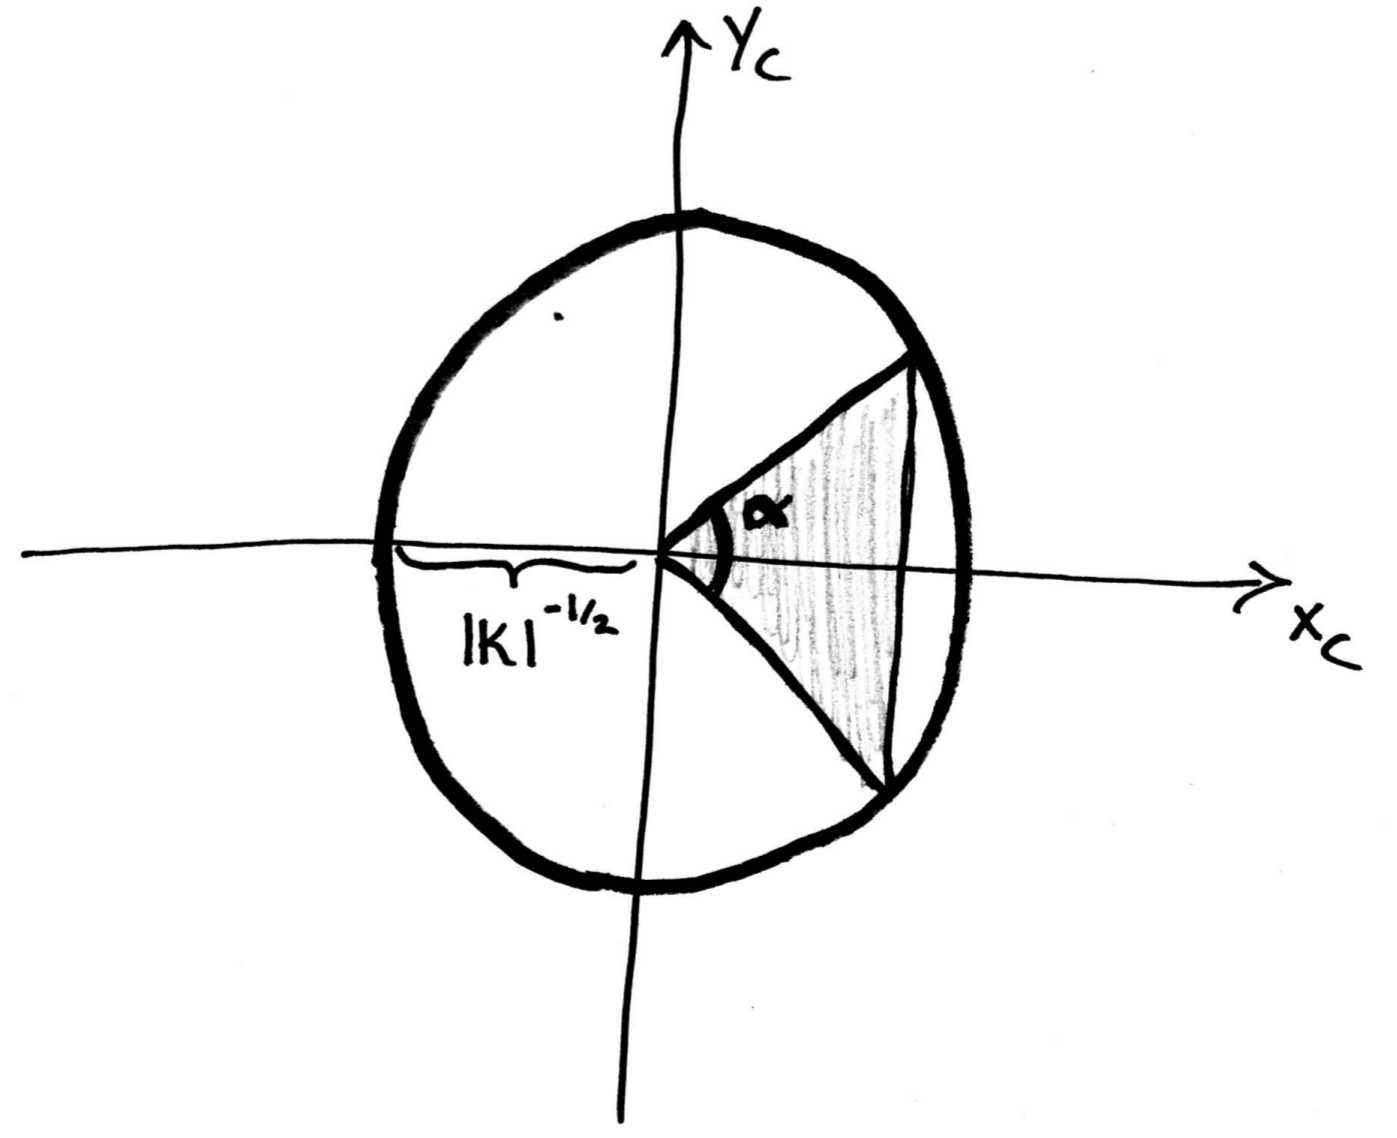
\includegraphics[width=3in]{diagramOfHyperbolicLune.png}
%\end{image}
%
%Notice that in both the Klein model and the Poincar\'e model, every line hits
%``the circle at infinity'' at two specific points.  This means we can talk about
%shapes with ``vertices at infinity''.
%
%\begin{definition}
%  We define an \dfn{$\boldsymbol\alpha$-lune} in hyperbolic geometry to be a
%  triangle with an angle of measure $\alpha$ where vertices opposite of $\alpha$
%  are at infinity.
%\end{definition}
%
%We have seen that
%\begin{align*}
%  \iint_{L_c} \sqrt{
%  \det
%  \begin{bmatrix}
%    \pp[X]{x_c}\bullet_K \pp[X]{x_c} & \pp[X]{y_c}\bullet_K \pp[X]{x_c} \\
%    \pp[X]{x_c}\bullet_K \pp[X]{y_c} & \pp[X]{y_c}\bullet_K \pp[X]{y_c}
%  \end{bmatrix}
%  }\d x_c\d y_c &=
%  \iint_{L_c} \sqrt{\det P_c}\d x_c\d y_c\\
%  &=\iint_{L_c} \left(K\left(x_c^2+y_c^2\right)+1\right)^{-3/2} \d x_c\d y_c.
%\end{align*}
%
%
%In what follows, we will assume that $K=-1$. This will simplify the
%computations somewhat. Once the mathematician is familiar with this
%case, the general case when $K<0$ will fall easily.
%
%
%\begin{problem}
%  Convert
%  \[
%  \iint_{L_c} \left(-\left(x_c^2+y_c^2\right)+1\right)^{-3/2} \d x_c\d y_c
%  \]
%  to polar coordinates and compute the integral.
%  \begin{hint}
%    Redraw the picture above with $\alpha = 2\beta$ and $K=-1$.
%  \end{hint}
%  \begin{hint}
%    Recall that to convert to polar coordinates, set
%    \begin{align*}
%      r &= \sqrt{x_c^2+y_c^2},\\
%      \theta &= \arctan(y_c/x_c),
%    \end{align*}
%    and replace $\d x_c\d y_c$ with $r\d r\d \theta$.
%  \end{hint}
%  \begin{hint}
%    At some point you may wish to use the following identities:
%    \[
%    \begin{split}
%      \cos^2\theta + \sin^2\theta &=1\\
%      \cos^2\theta &= 1-\sin^2\theta
%    \end{split}
%    \qquad
%    \begin{split}
%      \cos^2\beta + \sin^2\beta &=1\\
%      \cos^2\beta &= 1-\sin^2\beta
%    \end{split}
%    \]
%    So
%    \begin{align*}
%      \cos^2\theta - \cos^2\beta &= 1 - \sin^2\theta - \left(1-\sin^2\beta\right)\\
%      &= \sin^2\beta - \sin^2\theta.       
%    \end{align*}
%  \end{hint}
%  \begin{hint}
%    It may also be helpful to recall that when $a>0$,
%    \[
%    \int \frac{1}{\sqrt{a - u^2}} \d u = \arcsin\left(\frac{u}{\sqrt{a}}\right) + C.
%    \]
%  \end{hint}
%  \begin{hint}
%    Finally, as a gesture of friendship, I will tell you that you will
%    (hopefully!) deduce that this integral equals $\pi-\alpha$.
%  \end{hint}
%  \begin{freeResponse}
%    Write
%    \[
%    \int_{L_c} \left(-\left(x_c^2+y_c^2\right)+1\right)^{-3/2} \d x_c\d y_c
%    = \int_{-\beta}^\beta \int_0^{\frac{\cos \beta}{\cos\theta}}\left(-r^2+1\right)^{-3/2} r\d r\d \theta.
%    \]
%    Integrating this from the inside-out we find
%    \begin{align*}
%      &= \int_{-\beta}^\beta \eval{\left(-r^2+1\right)^{-1/2}}_0^{\frac{\cos \beta}{\cos\theta}}\d \theta\\
%      &= \int_{-\beta}^\beta \left(-\left(\frac{\cos \beta}{\cos\theta}\right)^2+1\right)^{-1/2}\d\theta - \eval{\theta}_{-\beta}^\beta\\
%      &= \int_{-\beta}^\beta \left(1-\frac{\cos^2 \beta}{\cos^2\theta}\right)^{-1/2}\d \theta -2\beta\\
%      &= \int_{-\beta}^\beta \left(\frac{\cos^2\theta - \cos^2 \beta}{\cos^2\theta}\right)^{-1/2} \d \theta-\alpha\\
%      &= \int_{-\beta}^\beta \frac{\cos\theta}{\sqrt{\cos^2\theta - \cos^2 \beta}}\d \theta - \alpha.
%    \end{align*}
%    Now apply a trigonometric substitution,
%    \[
%    = \int_{-\beta}^\beta \frac{\cos\theta}{\sqrt{\sin^2\beta - \sin^2 \theta}}\d \theta- \alpha,
%    \]
%    Using the hint above we see
%    \begin{align*}
%      &= \eval{\arcsin\left(\frac{\sin\theta}{\sin\beta}\right)}_{-\beta}^\beta - \alpha\\
%      &= \arcsin\left(\frac{\sin\beta}{\sin\beta}\right)- \arcsin\left(\frac{\sin(-\beta)}{\sin\beta}\right)- \alpha\\
%      &= \arcsin(1)-\arcsin(-1)-\alpha\\
%      &= \frac{\pi}{2}-\frac{-\pi}{2}-\alpha\\
%      &= \pi-\alpha.
%    \end{align*}
%  \end{freeResponse}
%\end{problem}


\section{Hyperbolic triangles}

We know that the area of a triangle on the $R$-sphere with angles
$\alpha$, $\beta$, and $\gamma$ is given by
\[
R^2(\alpha+\beta+\gamma - \pi).
\]
\begin{problem}
  Briefly (one paragraph or less) sketch the line of reasoning used to deduce the formula for
  the area of a triangle on the $R$-sphere.
\end{problem}

\begin{problem}
In one paragraph or less, explain why the formula for the area of a triangle on the $R$ sphere is the same in Euclidean coordinates and in $K$-warped coordinates.
\end{problem}

\begin{problem}
 Use $K$-warped coordinates to give the formula for the area of a triangle on the hyperbolic plane, where $K<0$.
\end{problem}

\begin{definition}
  An \dfn{ideal triangle} is a triangle in hyperbolic geometry with all of
  its vertices at infinity.
\end{definition}

\begin{problem}
  Calculate the area of the shaded hyperbolic triangle
  
\begin{image}
 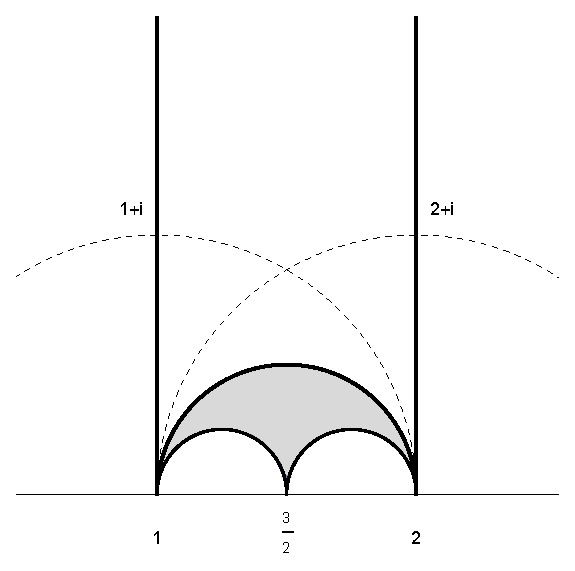
\includegraphics{fareycell}
 
\end{image}
  \end{problem}


\begin{definition}
  An \dfn{ideal $\boldsymbol{n}$-gon} is an $n$-gon in hyperbolic
  geometry with its vertices at infinity.
\end{definition}

\begin{problem}
Use induction to derive a formula for the area of any ideal $n$-gon 
hyperbolic geometry.
\end{problem}

%\begin{problem}
%  Use the diagrams below
%  \begin{image}
%  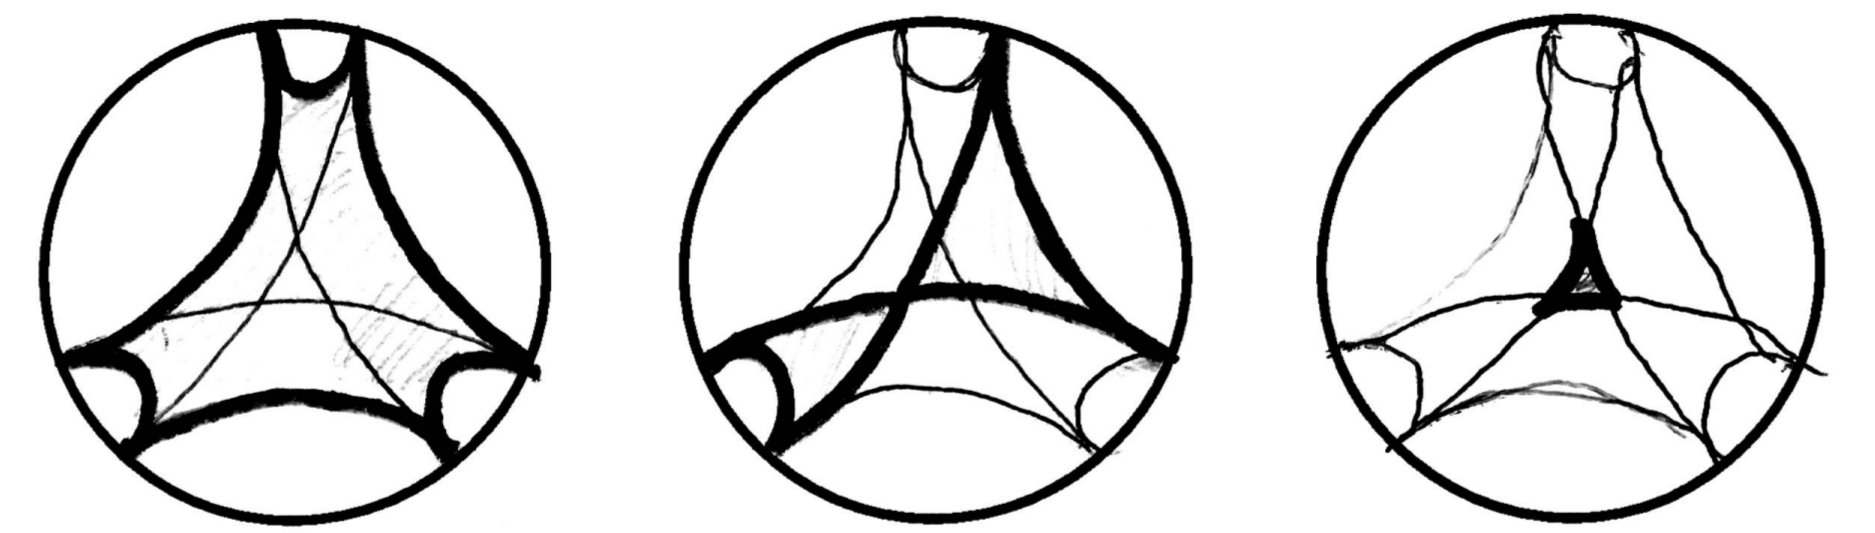
\includegraphics[width=4in]{diagramHex.png}
%  \end{image}
%  to help compute the area of a triangle in hyperbolic geometry.
%  \begin{hint}
%    Make your own drawings inspired by those above.
%  \end{hint}
%  \begin{hint}
%    Make sure your computation is general: start with an arbitrary triangle and
%    explain how you can fill in the rest of the diagram.
%  \end{hint}
%\end{problem}


\begin{problem}
Summarize the results from this section. In particular, rephrase the results in your own words and indicate which
results follow from the others.
\begin{freeResponse}
\end{freeResponse}
\end{problem}




\end{document}
